\documentclass[10pt, aspectratio=169]{beamer}

% --- IMPOSTAZIONI TEMPLATE UNIFI ---
\usetheme{sintef} 
\titlebackground*{assets/background} % <-- IL COMANDO MAGICO MANCANTE!

% Pacchetti utili
\usepackage[utf8]{inputenc}
\usepackage{amsmath}
\usepackage{graphicx}
\usepackage{booktabs}
\usepackage{appendixnumberbeamer}
\usepackage{verbatim}

% --- METADATI DELLA COPERTINA ---
\title[Hybrid Quantum-Classical Architecture]{Hybrid Quantum-Classical Architecture \\ for Solving Large-Scale QUBO Problems}
\subtitle{A Divide et Impera Approach}

% Pulito, senza doppi backslash iniziali e senza \vspace forzati che sballano il layout
\author{\texorpdfstring{\\ \vspace{0.5cm} Candidate: Giacomo Orsucci \\ \vspace{0.2cm} Supervisors: Dr. B. Picano, Prof. R. Fantacci \\ Co-supervisor: Dr. C. Cicconetti}{Giacomo Orsucci}}

\date{Academic Year 2025/2026}

\begin{document}
\maketitle
\begin{frame}{Research Context and Scholarship}
    \framesubtitle{Institute of Informatics and Telematics (CNR) and Neutral Atoms}
    
    % Logo IIT in alto a destra
    \begin{tikzpicture}[remember picture,overlay]
        \node[anchor=north east, xshift=-0.5cm, yshift=-0.2cm] at (current page.north east) {
\includegraphics[height=0.9cm]{img/IIT.png}};
    \end{tikzpicture}
    
    % Margine ridotto per tirare i riquadri più in alto
    \vspace{0.1cm}
    
    % [T] allinea le colonne in alto
    \begin{columns}[T]
        
        % COLONNA SINISTRA: L'Hardware
        \begin{column}{0.48\textwidth}
            \begin{block}{The Hardware}
                % Contenitore fisso alto 4.8cm con contenuto centrato verticalmente [c]
                \begin{minipage}[c][4.8cm][c]{\linewidth}
                    \centering
                    % L'immagine non verrà mai tagliata: si adatta senza superare i bordi
                    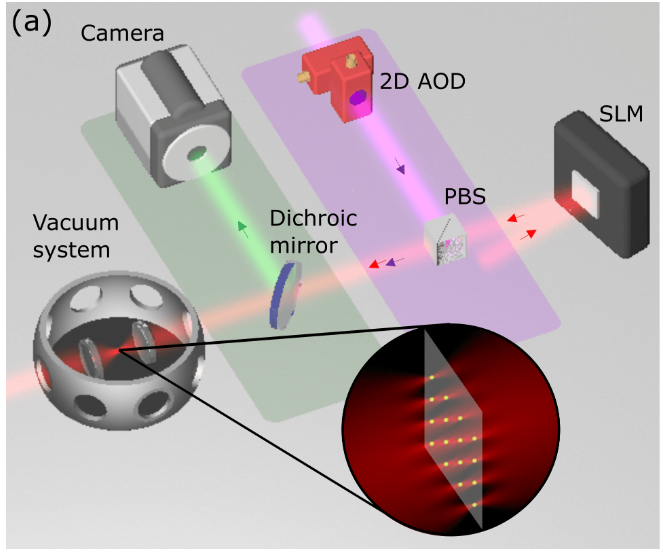
\includegraphics[width=\linewidth, height=4.6cm, keepaspectratio]{img/principal_compo_QPU.png}
                \end{minipage}
            \end{block}
        \end{column}
        
        % COLONNA DESTRA: Le Topologie Spaziali
        \begin{column}{0.48\textwidth}
            \begin{block}{The Challenge}
                % Contenitore identico per avere i due blocchi alti uguali al millimetro
                \begin{minipage}[c][4.8cm][c]{\linewidth}
                    \centering
                    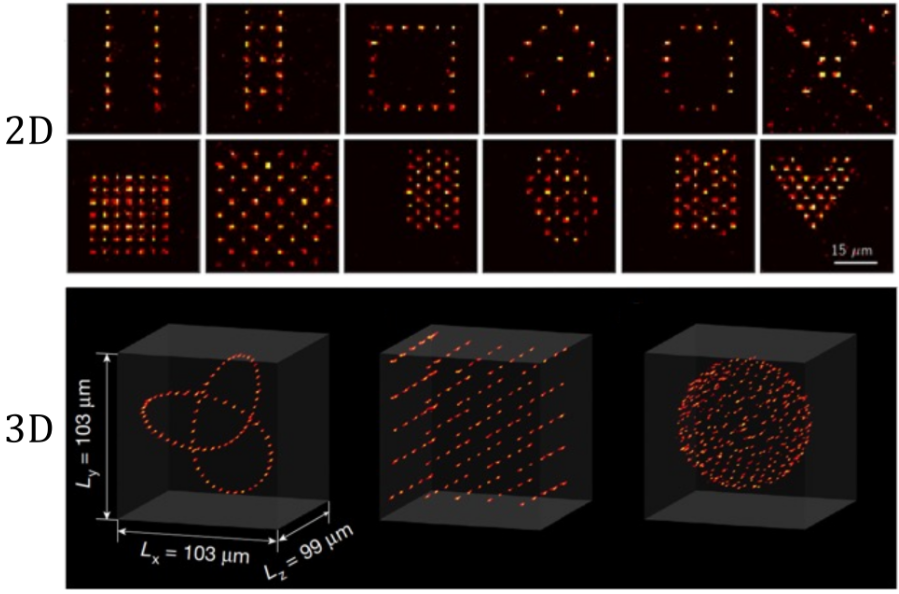
\includegraphics[width=\linewidth, height=4.6cm, keepaspectratio]{img/2D-3D_neutral_atom_reg.png}
                \end{minipage}
            \end{block}
        \end{column}
        
    \end{columns}
    
    \vfill
    

    
    \vspace{0.1cm}
\end{frame}


\begin{frame}{QUBO problems}
    \framesubtitle{QUBO formulation}
    
    \vfill % Spinge l'equazione verso il centro
    
    {\Large % Aumenta la dimensione del font matematico
    \begin{equation}
        \min_{x \in \{0,1\}^n} f(x) = x^T Q x = \sum_{i=1}^{n} \sum_{j=1}^{n} Q_{i,j} x_i x_j
    \end{equation}
    }
    
    \vfill % Spinge l'equazione verso il centro
    
\end{frame}


% SLIDE 1: Equazione intera e mapping
\begin{frame}{Physical Formulation}
    \framesubtitle{QUBO to Ising Hamiltonian Mapping (1/3)}
    
    
    \vfill
    
    {\Large
    \begin{equation}
        \hat{\mathcal{H}}(t) = \hbar\sum_{i=1}^{N}\left(\frac{\Omega(t)}{2}\hat{\sigma}_{i}^{x}-\delta(t)\hat{n}_{i}\right) + \sum_{i<j}\frac{C_{6}}{|r_{i}-r_{j}|^{6}}\hat{n}_{i}\hat{n}_{j}
    \end{equation}
    }
    
    \vfill
\end{frame}


% SLIDE 2: Focus sul primo termine (Lineare/Laser)
\begin{frame}{Physical Formulation}
    \framesubtitle{Single-Atom Driving: Linear Terms (2/3)}
    
    \vfill
    
    {\Large
    \begin{equation}
        \hat{\mathcal{H}}(t) = \fcolorbox{red}{white}{$\displaystyle \hbar\sum_{i=1}^{N}\left(\frac{\Omega(t)}{2}\hat{\sigma}_{i}^{x}-\delta(t)\hat{n}_{i}\right)$} + \textcolor{gray}{\sum_{i<j}\frac{C_{6}}{|r_{i}-r_{j}|^{6}}\hat{n}_{i}\hat{n}_{j}}
    \end{equation}
    }
    
    \vfill
\end{frame}


% SLIDE 3: Focus sul secondo termine (Quadratico/Interazione)
\begin{frame}{Physical Formulation}
    \framesubtitle{Pairwise Interactions: Quadratic Penalties (3/3)}
    
    \vfill
    
    {\Large
    \begin{equation}
        \hat{\mathcal{H}}(t) = \textcolor{gray}{\hbar\sum_{i=1}^{N}\left(\frac{\Omega(t)}{2}\hat{\sigma}_{i}^{x}-\delta(t)\hat{n}_{i}\right)} + \fcolorbox{red}{white}{$\displaystyle \sum_{i<j}\frac{C_{6}}{|r_{i}-r_{j}|^{6}}\hat{n}_{i}\hat{n}_{j}$}
    \end{equation}
    }
    
    \vfill
\end{frame}


\begin{frame}{The Embedding Problem}
    \framesubtitle{Hardware Constraints (Pasqal \textit{Jade})}
    
    \vspace{0.2cm}
    
    % Dashboard a 3 colonne per i vincoli fisici
    \begin{columns}[T]
        
        % Vincolo 1: Raggio
        \begin{column}{0.31\textwidth}
            \begin{block}{Maximum Radius}
                \centering
                \vspace{0.2cm}
                {\Large \textbf{50.0 $\mu$m}} \\[0.1cm]
                \footnotesize Register boundary ($R_{\text{max}}$)
                \vspace{0.15cm}
            \end{block}
        \end{column}
        
        % Vincolo 2: Distanza
        \begin{column}{0.31\textwidth}
            \begin{block}{Minimum Distance}
                \centering
                \vspace{0.2cm}
                {\Large \textbf{4.0 $\mu$m}} \\[0.1cm]
                \footnotesize Diffraction limit ($d_{\text{min}}$)
                \vspace{0.15cm}
            \end{block}
        \end{column}
        
        % Vincolo 3: Laser
        \begin{column}{0.34\textwidth}
            \begin{block}{Global Laser}
                \centering
                \vspace{0.2cm}
                {\Large \textbf{$\Omega(t)$ \& $\delta(t)$}} \\[0.1cm]
                \footnotesize Uniform parameterization
                \vspace{0.15cm}
            \end{block}
        \end{column}
        
    \end{columns}
    
    \vfill 
    
    % Immagine del polso laser in basso
    \begin{center}
        % Sostituisci col nome esatto della tua immagine
        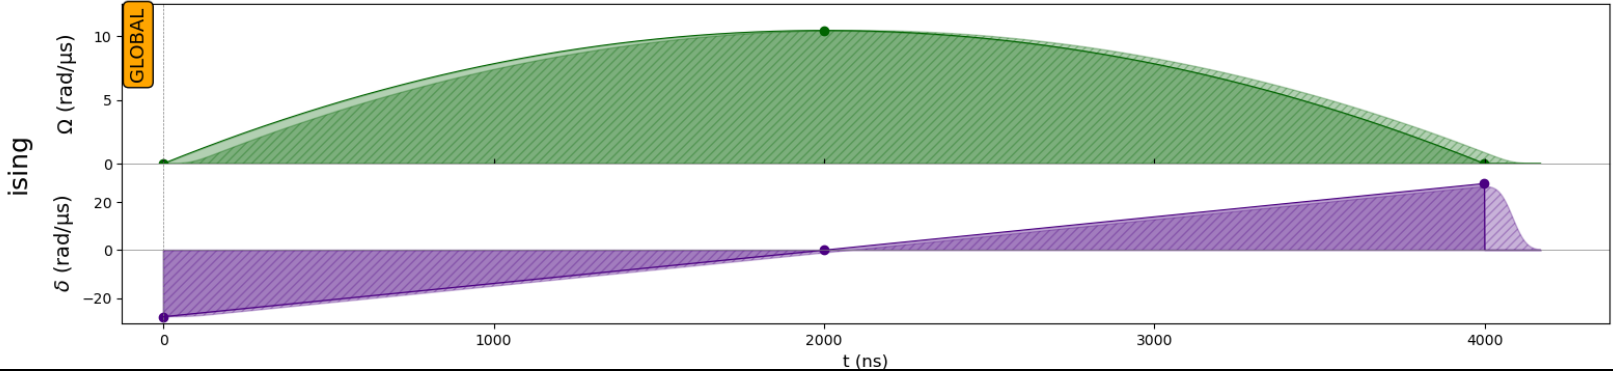
\includegraphics[width=0.95\linewidth]{img/ray_params.png}
    \end{center}
    
    \vspace{0.2cm}
\end{frame}

\begin{frame}{Embeddable problems: Unit Disk Graphs}
    \framesubtitle{UDG Problems formalization and visualization}
    \begin{figure}[htbp]
    \centering
    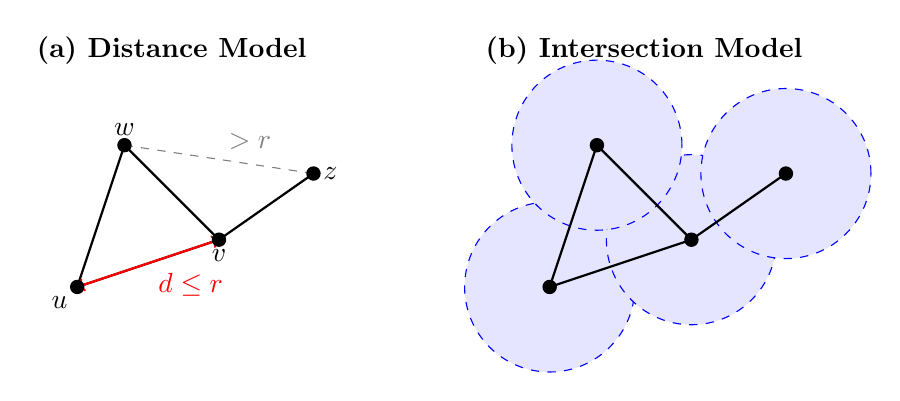
\begin{tikzpicture}[scale=1.2]
        % --- Pannello Sinistro: Distance Model ---
        \node at (1, 2.5) {\textbf{(a) Distance Model}};

        % definizione dei nodi (punti)
        \coordinate (A) at (0, 0);
        \coordinate (B) at (1.5, 0.5);
        \coordinate (C) at (0.5, 1.5);
        \coordinate (D) at (2.5, 1.2);

        % Disegno degli archi validi (distanza <= r)
        \draw[thick] (A) -- (B) -- (C) -- (A);
        \draw[thick] (B) -- (D);

        % Disegno di un arco non valido per mostrare che la distanza > r
        \draw[dashed, gray] (C) -- (D) node[midway, above right] {$> r$};

        % Etichetta della distanza <= r
        \draw[<->, red, thick] (A) -- (B) node[midway, below right] {$d \leq r$};

        % Disegno dei pallini dei nodi
        \filldraw (A) circle (2pt) node[below left] {$u$};
        \filldraw (B) circle (2pt) node[below] {$v$};
        \filldraw (C) circle (2pt) node[above] {$w$};
        \filldraw (D) circle (2pt) node[right] {$z$};

        % --- Pannello Destro: Intersection Model ---
        \begin{scope}[xshift=5cm] % Sposto tutto a destra di 5cm
        \node at (1, 2.5) {\textbf{(b) Intersection Model}};

        \coordinate (A2) at (0, 0);
        \coordinate (B2) at (1.5, 0.5);
        \coordinate (C2) at (0.5, 1.5);
        \coordinate (D2) at (2.5, 1.2);

        % Raggio dei cerchi (r/2)
        \def\rad{0.9}

        % Disegno i cerchi (le "aree di influenza")
        \draw[fill=blue!10, draw=blue, dashed] (A2) circle (\rad);
        \draw[fill=blue!10, draw=blue, dashed] (B2) circle (\rad);
        \draw[fill=blue!10, draw=blue, dashed] (C2) circle (\rad);
        \draw[fill=blue!10, draw=blue, dashed] (D2) circle (\rad);

        % Disegno gli archi dove i cerchi si sovrappongono
        \draw[thick] (A2) -- (B2) -- (C2) -- (A2);
        \draw[thick] (B2) -- (D2);

        \filldraw (A2) circle (2pt);
        \filldraw (B2) circle (2pt);
        \filldraw (C2) circle (2pt);
        \filldraw (D2) circle (2pt);
        \end{scope}
    \end{tikzpicture}
    \label{fig:udg_models}
    \end{figure}
\end{frame}


% SLIDE 5
\begin{frame}{Baseline}
    \framesubtitle{Pipeline Overview}
    \begin{figure}[htbp]
        \centering
        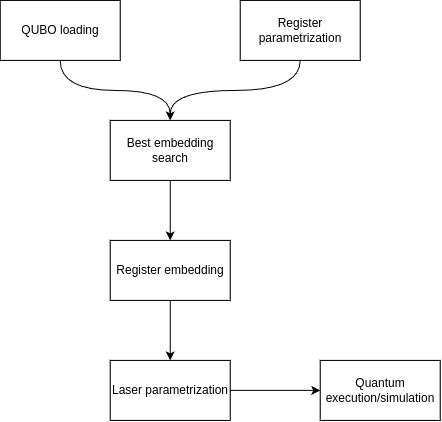
\includegraphics[width=0.4\textwidth]{img/base_pipeline.png} 
    \end{figure}
\end{frame}

\begin{comment}

% SLIDE 6
\begin{frame}{Embedding search}
    \framesubtitle{Genetic Algorithms \& Simulated Annealing}
    We implemented a baseline hybrid pipeline to test monolithic embeddings:
    \begin{itemize}
        \item \textbf{Genetic Algorithms (GA):} Evolving 2D coordinates. Works for small instances, but crossover operations are physically destructive on dense spatial layouts.
        \item \textbf{Simulated Annealing (SA):} A single-trajectory thermodynamic approach enhanced with a \textbf{GRASP initialization} and zero-temperature \textbf{Quenching}.
    \end{itemize}
    \vspace{0.3cm}
    \textbf{The Evaluation Metric:} A custom Improved Topological MAE fitness function that handles maximum physical potential clipping and bounds crossover.
\end{frame}

% SLIDE 9: Transition & Legend for Results
\begin{frame}{Baseline Results Roadmap}
\framesubtitle{How to Read the Experimental Data}
    The following slides evaluate the scaling limits of monolithic embeddings (GA vs. SA). Each test is presented in a standardized dual-panel layout:
    
    \vspace{0.4cm}
    \begin{columns}[T]
        % LEFT COLUMN
        \begin{column}{0.48\textwidth}
            \textbf{Left Panel: Spatial Embedding}
            \begin{itemize}
                \item The physical 2D coordinate layout found.
                \item Light shaded areas represent the physical atomic radius, visually confirming compliance with the minimum distance constraint ($d_{min}$).
            \end{itemize}
        \end{column}
        
        % RIGHT COLUMN
        \begin{column}{0.48\textwidth}
            \textbf{Right Panel: Analog Quantum Readout}
            \begin{itemize}
                \item The probability distribution of the actual bitstrings measured after the adiabatic emulation.
                \item \textbf{\textcolor{green}{Green Bars:}} The \textit{true mathematical ground states}, verified via exact classical benchmarking.
                \item \textbf{\textcolor{blue}{Blue Bars:}} Sub-optimal measurements, representing excited states or false local minima.
            \end{itemize}
        \end{column}
    \end{columns}
\end{frame}
\end{comment}
% SLIDE 7
\begin{frame}{Baseline Results}
\framesubtitle{GA on a 10x10 Instance}
    \begin{columns}[c] 
        \begin{column}{0.38\textwidth}
            \centering
            \textbf{Spatial Embedding} \\
            \vspace{0.2cm}
            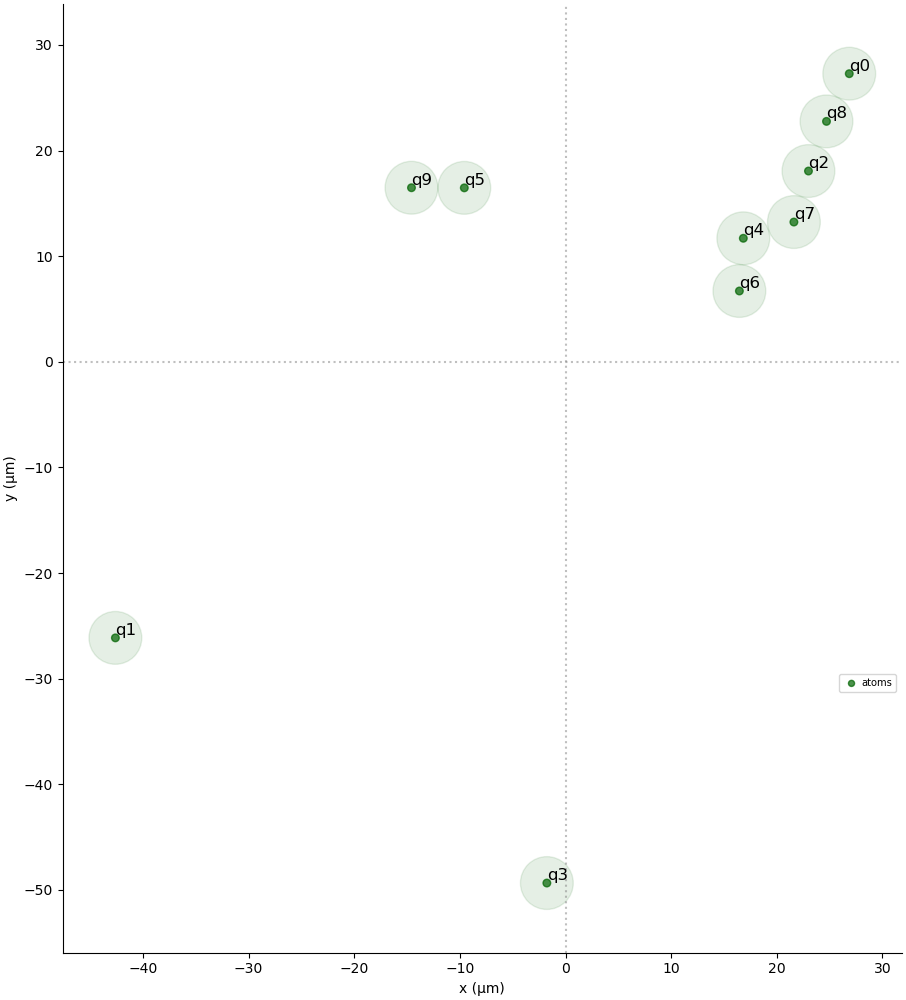
\includegraphics[width=\linewidth]{img/reg_10x10_d3.0.png} 
        \end{column}
        
        \begin{column}{0.6\textwidth}
            \centering
            \textbf{Quantum Readout} \\
            \vspace{0.2cm}
            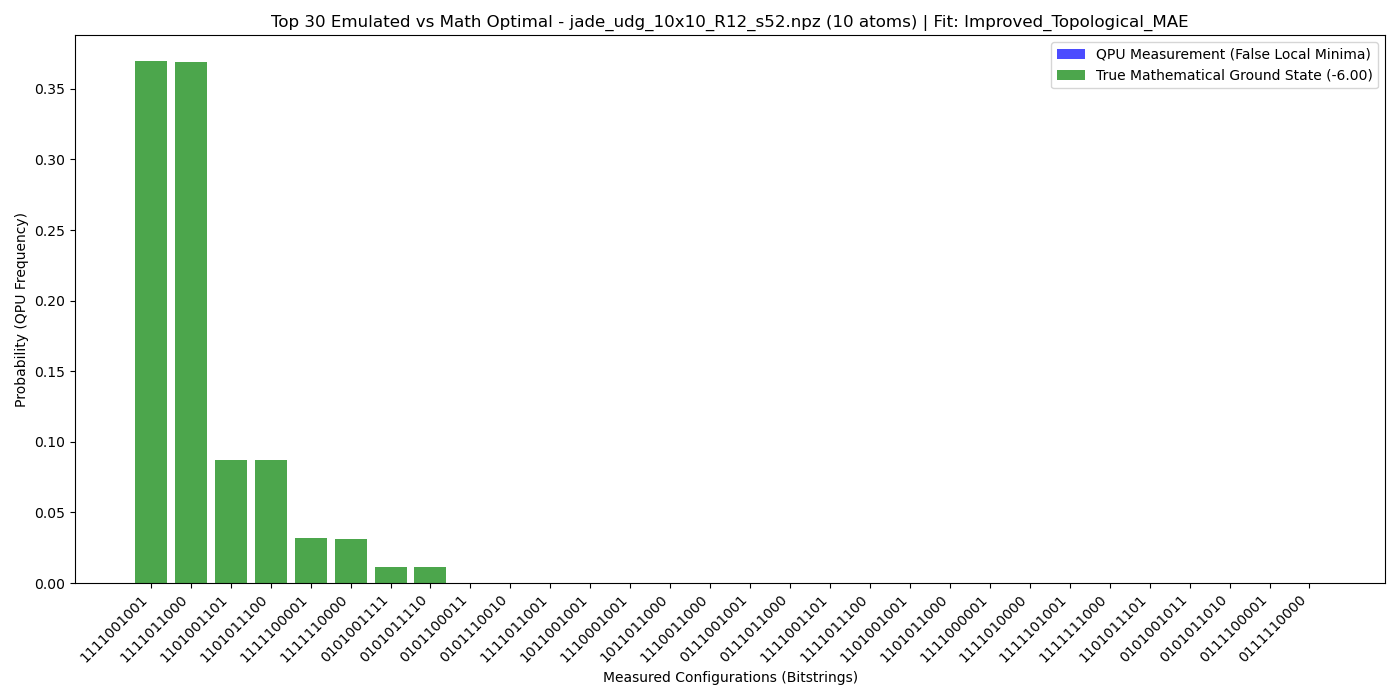
\includegraphics[width=\linewidth]{img/res_10x10_d3.0.png} 
        \end{column}
    \end{columns}
\end{frame}

% SLIDE 8
\begin{frame}{Baseline Results}
\framesubtitle{Scaling limits: GA on a 15x15 Instance}    \begin{columns}[c] 
        \begin{column}{0.38\textwidth}
            \centering
            \textbf{Spatial Embedding} \\
            \vspace{0.2cm}
            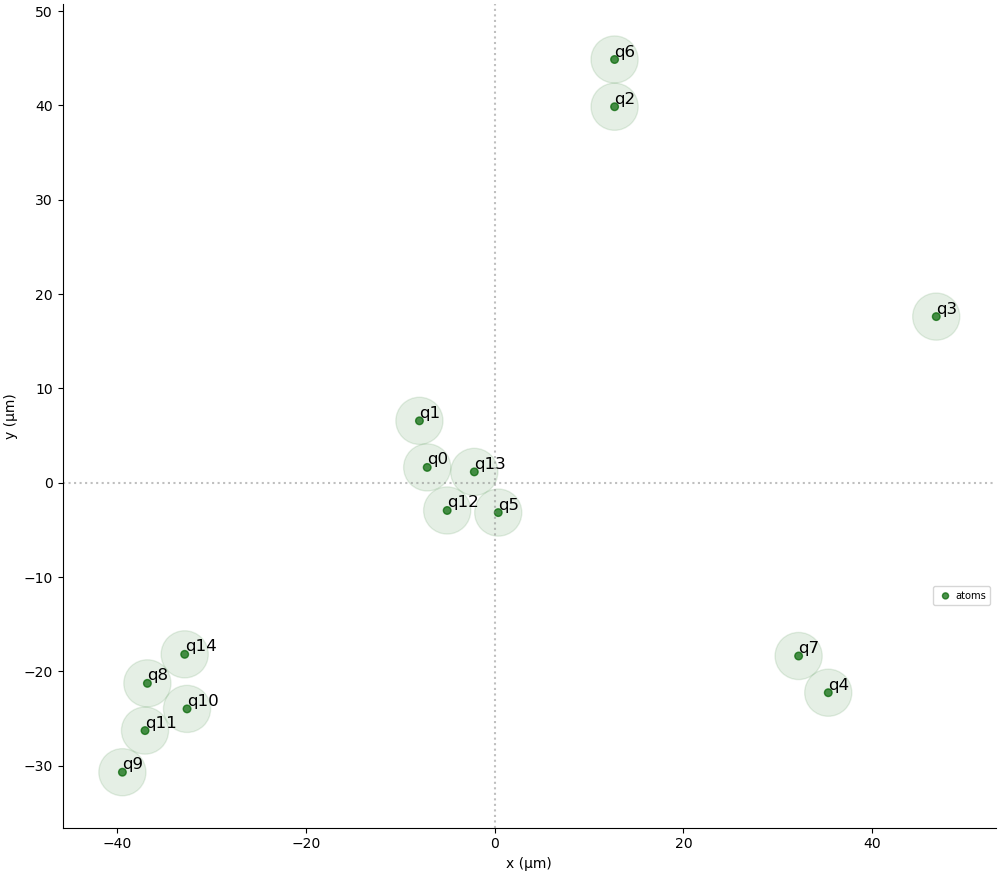
\includegraphics[width=\linewidth]{img/reg_15x15.png} 
        \end{column}
        
        \begin{column}{0.6\textwidth}
            \centering
            \textbf{Quantum Readout} \\
            \vspace{0.2cm}
            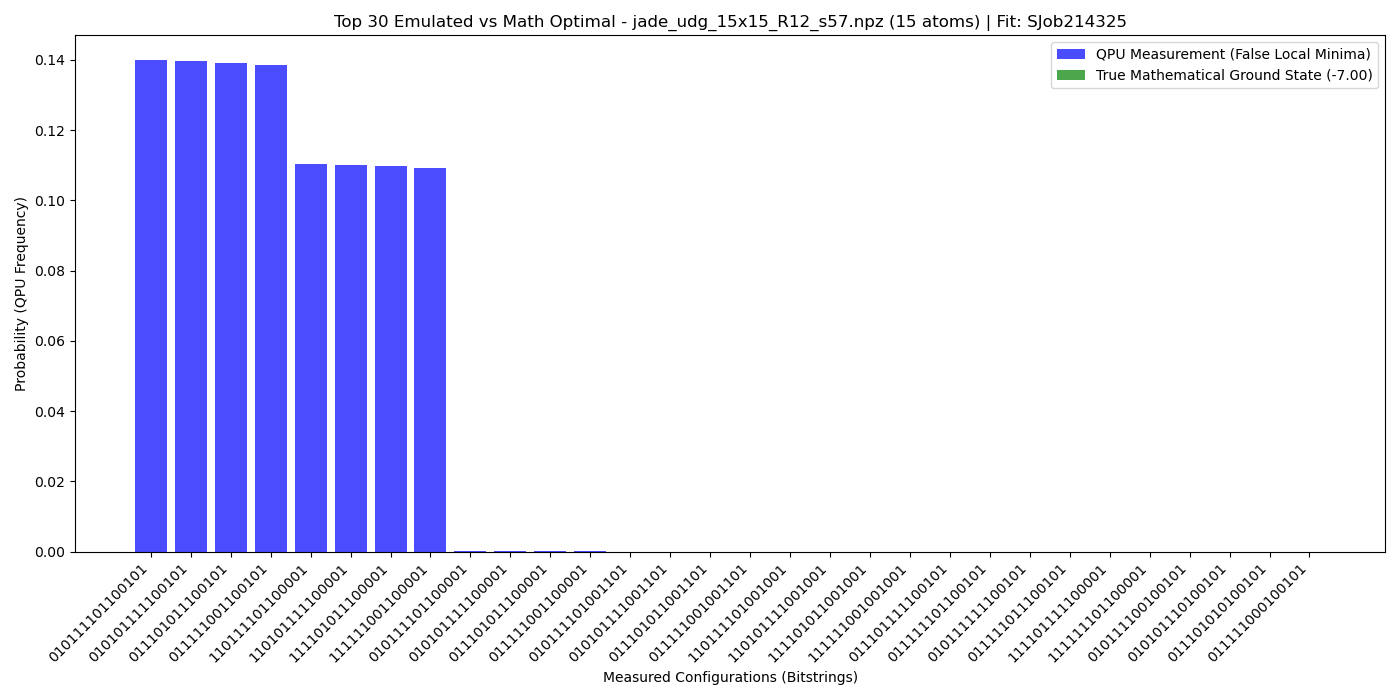
\includegraphics[width=\linewidth]{img/res_15x15.png} 
        \end{column}
    \end{columns}
\end{frame}

% SLIDE 9
\begin{frame}{Baseline Results}
\framesubtitle{SA on a 15x15 Instance}    \begin{columns}[c] 
        \begin{column}{0.38\textwidth}
            \centering
            \textbf{Spatial Embedding} \\
            \vspace{0.2cm}
            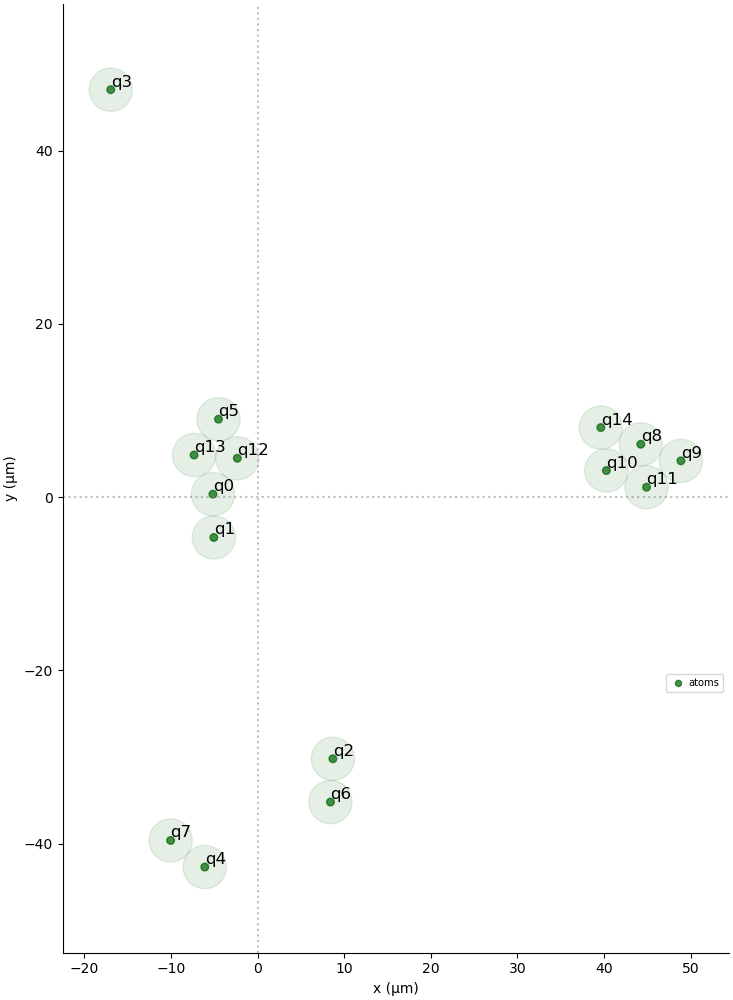
\includegraphics[width=\linewidth, height=1.2\textwidth]{img/reg_15x15_SA.png} 
        \end{column}
        
        \begin{column}{0.6\textwidth}
            \centering
            \textbf{Quantum Readout} \\
            \vspace{0.2cm}
            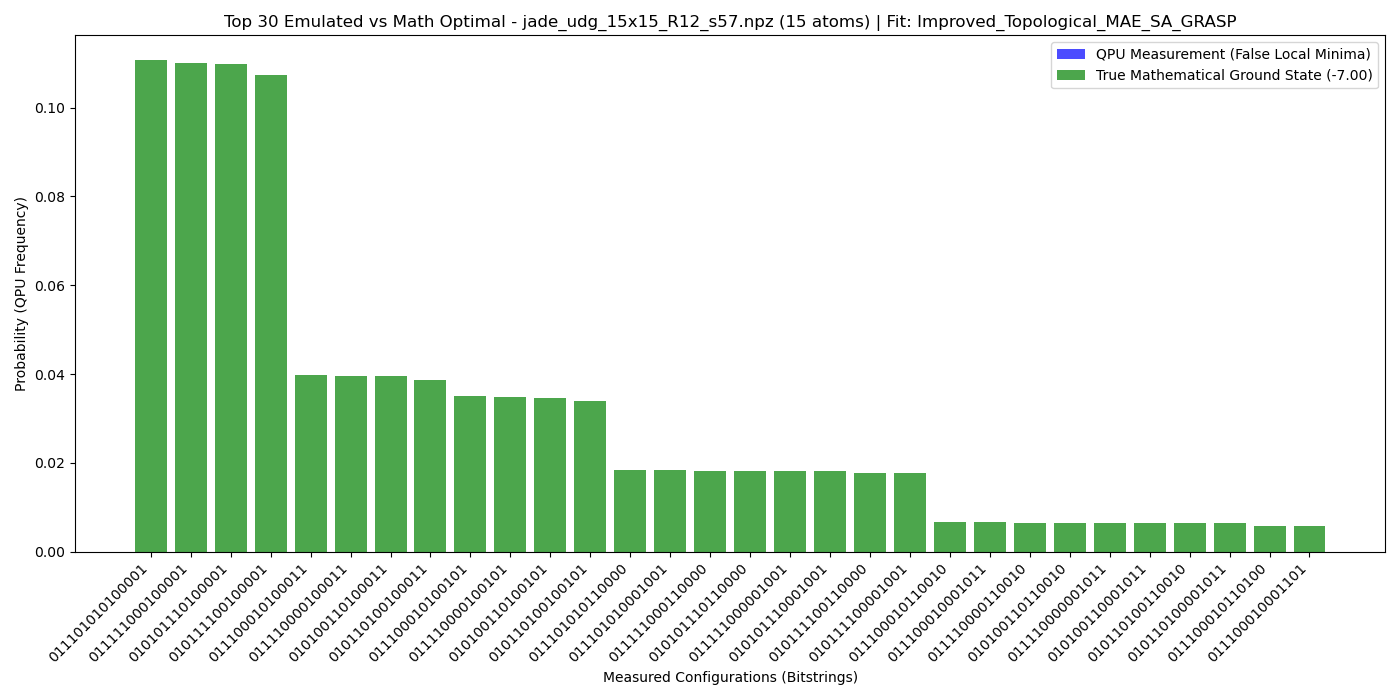
\includegraphics[width=\linewidth]{img/res_15x15_SA.png} 
        \end{column}
    \end{columns}
\end{frame}

% SLIDE 10
\begin{frame}{Baseline Results}
\framesubtitle{SA on a 20x20 Instance}    \begin{columns}[c] 
        \begin{column}{0.38\textwidth}
            \centering
            \textbf{Spatial Embedding} \\
            \vspace{0.2cm}
            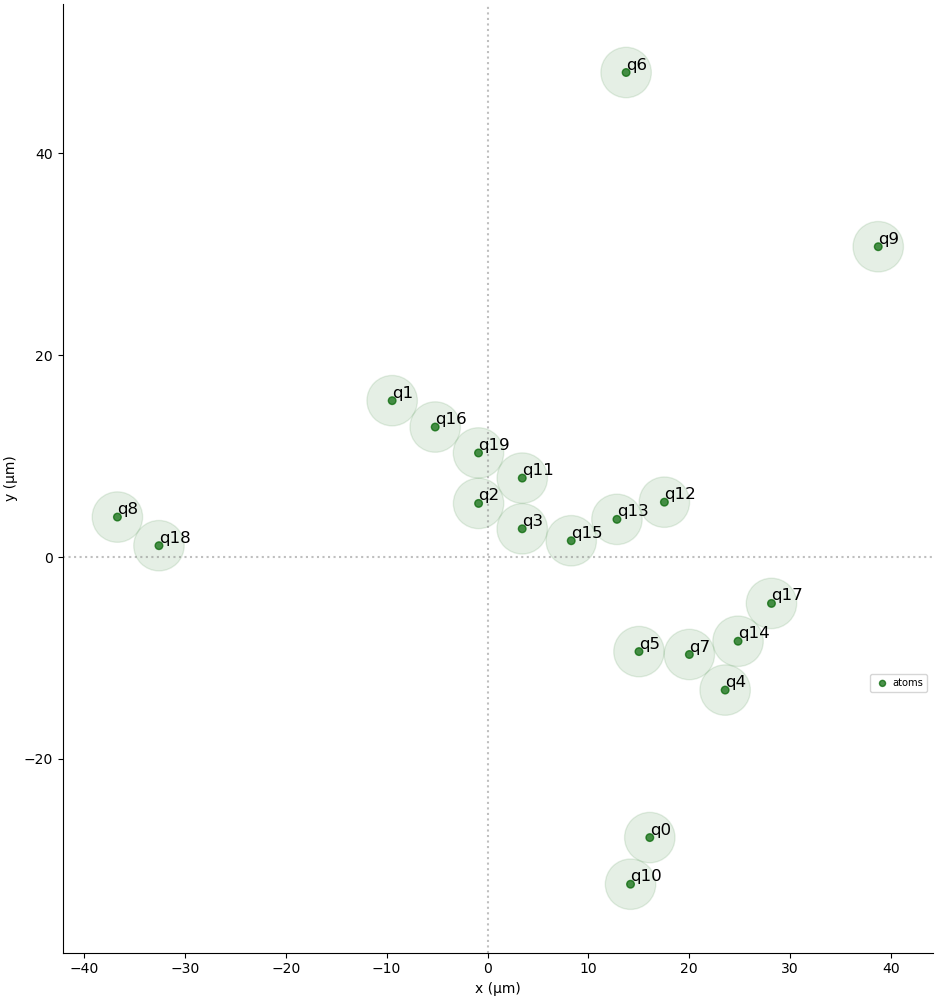
\includegraphics[width=\linewidth]{img/reg_20x20_d3.0.png} 
        \end{column}
        
        \begin{column}{0.6\textwidth}
            \centering
            \textbf{Quantum Readout} \\
            \vspace{0.2cm}
            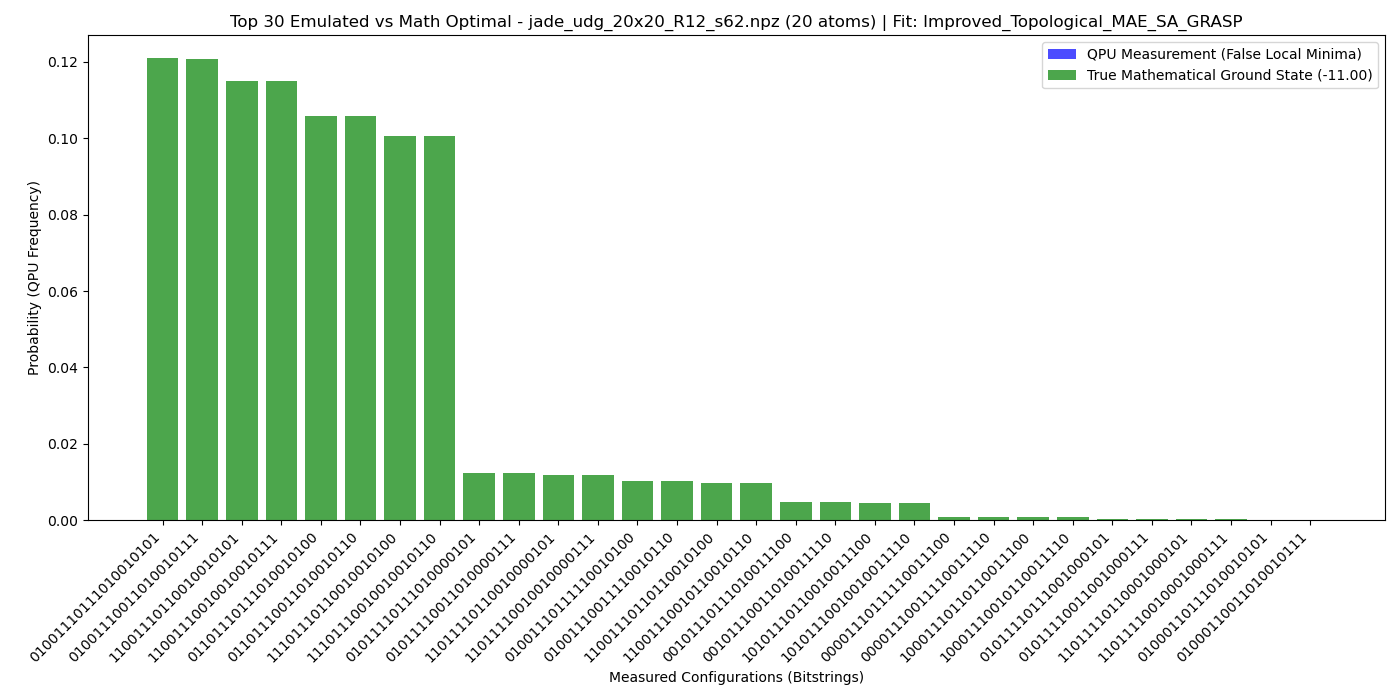
\includegraphics[width=\linewidth]{img/res_20x20_d3.0.png} 
        \end{column}
    \end{columns}
\end{frame}

% SLIDE 11
\begin{frame}{Baseline Results}
\framesubtitle{SA on a more difficult 20x20 Instance}    \begin{columns}[c] 
        \begin{column}{0.38\textwidth}
            \centering
            \textbf{Spatial Embedding} \\
            \vspace{0.2cm}
            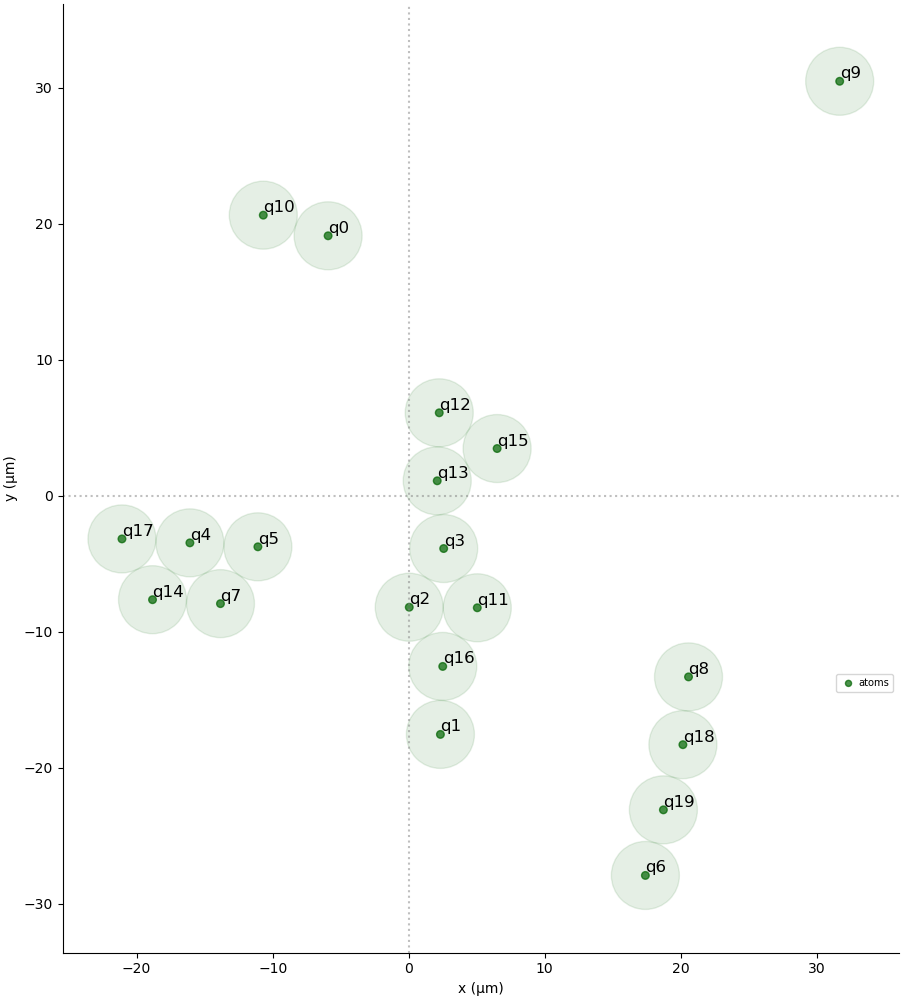
\includegraphics[width=\linewidth]{img/reg_20x20_d5.0_third.png} 
        \end{column}
        
        \begin{column}{0.6\textwidth}
            \centering
            \textbf{Quantum Readout} \\
            \vspace{0.2cm}
            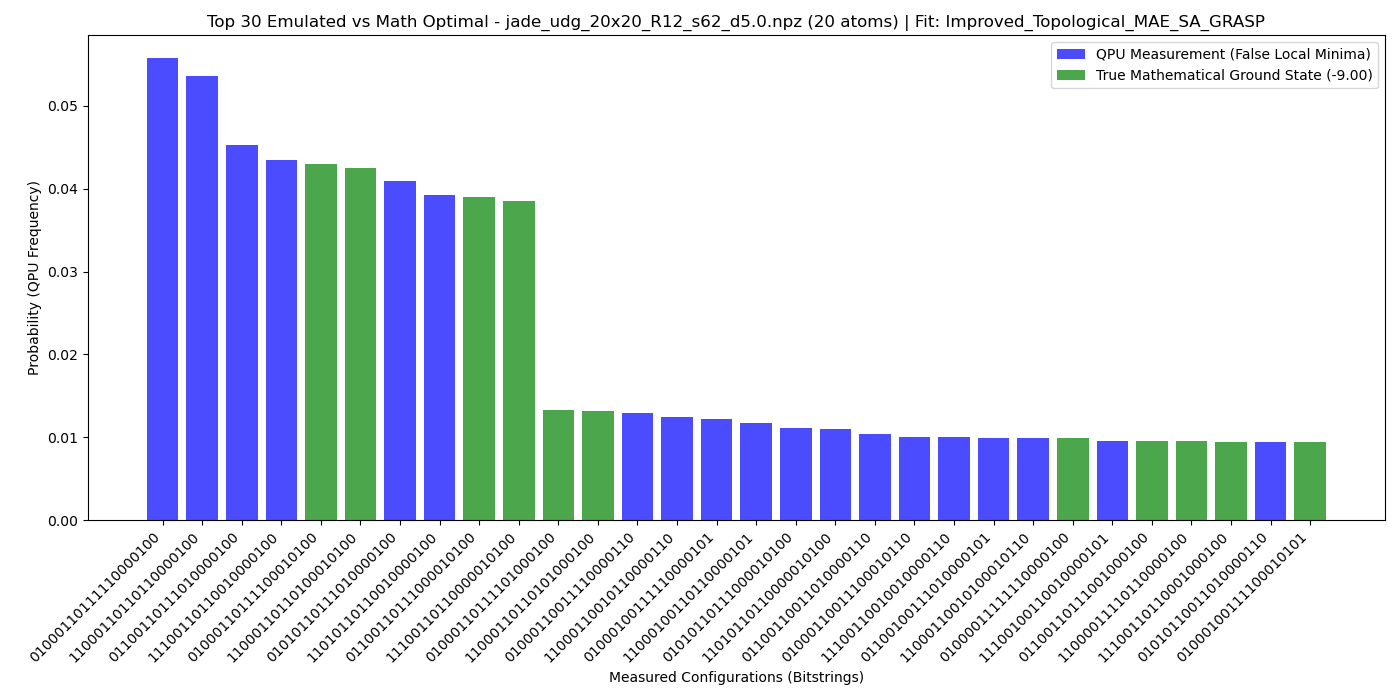
\includegraphics[width=\linewidth]{img/res_20x20_d5.0_third.png} 
        \end{column}
    \end{columns}
\end{frame}

\begin{frame}{The Scalability Wall}
    \framesubtitle{The Operational Breaking Point}
    
    \vspace{0.4cm}
    
    \begin{columns}[T]
        
        % PANNELLO SINISTRO: Il Problema (Rosso scuro/Marrone per indicare il limite)
        \begin{column}{0.48\textwidth}
            \begin{block}{The Monolithic Bottleneck}
                \vspace{0.2cm}
                \centering
                \textbf{Spatial Curse of Dimensionality}\\[0.3cm]
                \raggedright
                \vspace{0.2cm}
                \begin{itemize}
                    \item \textbf{GA} fails on $15 \times 15$ instances.
                    \item \textbf{SA} degrades severely on $20 \times 20$ instances.
                \end{itemize}
                \vspace{0.2cm}
            \end{block}
        \end{column}
        
        % PANNELLO DESTRO: La Soluzione (Blu/Verde per indicare la via d'uscita)
        \begin{column}{0.48\textwidth}
            \begin{block}{The Required Paradigm Shift}
                \vspace{0.2cm}
                \centering
                \textbf{From Global to Distributed}\\[0.3cm]
                \raggedright
            The embedding of larger problems demands a structural \textbf{paradigm shift}.\\
                
                \vspace{0.55cm} % Spaziatura per bilanciare l'altezza con il pannello sinistro
            \end{block}
        \end{column}
        
    \end{columns}
    
\end{frame}



% SLIDE 13
\begin{frame}{The \textit{Divide et Impera} Approach}
\framesubtitle{Partitioning Phase}
    \vspace{0.2cm}
    \begin{center}
        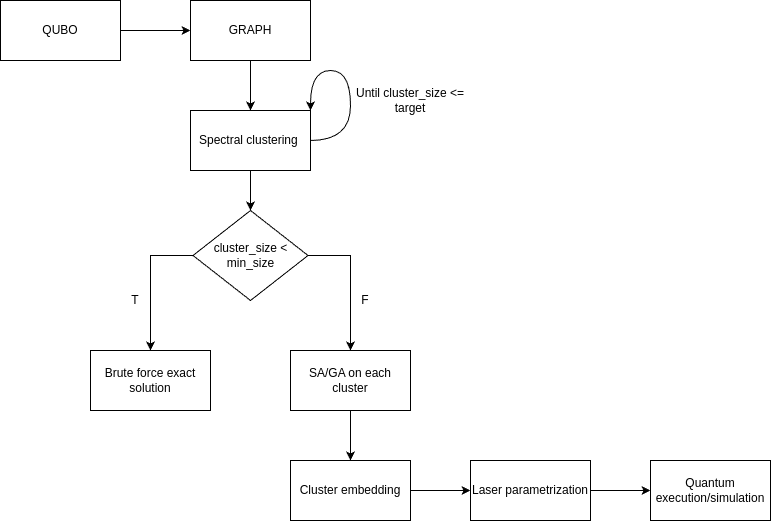
\includegraphics[width=0.6\textwidth]{img/Divide_et_impera_pipeline.png} 
    \end{center}
    \vspace{0.1cm}
\end{frame}

% SLIDE 14
\begin{frame}{The \textit{Divide et Impera} Approach}
\framesubtitle{Merging Phase}
   \begin{center}
        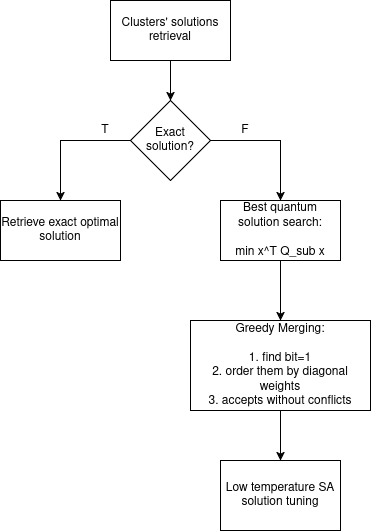
\includegraphics[width=0.3\textwidth, height=0.9\textheight]{img/Retrieval-merging.png} 
    \end{center} 
\end{frame}

% SLIDE 15
\begin{frame}{Experimental Results}
\framesubtitle{Extreme saturation: Denser $100 \times 100$ Instance}
\framesubtitle{Pushing the frontier: $100 \times 100$ Instance}
    \textbf{Target:} Pushing the operational frontier on a highly dense UDG QUBO matrix.
    \vspace{0.4cm}

    \begin{columns}[T]
        \begin{column}{0.48\textwidth}
            \textbf{1. Topological Profile \& Routing}
            \vspace{0.2cm}
            
            \resizebox{\linewidth}{!}{
            \begin{tabular}{lr}
                \toprule
                \textbf{Metric} & \textbf{Value} \\
                \midrule
                Variables (Nodes) & $100$ \\
                Graph Density & $4.8\%$ \\
                Max Node Degree & $10$ \\
                \midrule
                Total Sub-clusters & $10$ \\
                Cluster Sizes & From $2$ to $15$ nodes \\
                Execution Routing & $1$ Exact, $9$ QPU (SA) \\
                \bottomrule
            \end{tabular}
            }
        \end{column}
        
        \begin{column}{0.5\textwidth}
            \textbf{2. Energy Convergence}
            \vspace{0.2cm}
            
            \resizebox{\linewidth}{!}{
            \begin{tabular}{lc}
                \toprule
                \textbf{Reconstruction Phase} & \textbf{Global Energy} \\
                \midrule
                Baseline Greedy (No filter) & $-29.0$ \\
                Filtered Greedy (Noise mitigation) & $-35.0$ \\
                \midrule
                \textbf{Final Low-Temp SA Refinement} & $\mathbf{-37.0^*}$ \\
                \bottomrule
            \end{tabular}
            }
            
            \vspace{0.4cm}
            {\small \textit{* Perfectly matches the true global minimum independently approximated via D-Wave benchmark.}}
        \end{column}
    \end{columns}
\end{frame}

% SLIDE 16
\begin{frame}{Experimental Results}
\framesubtitle{Extreme saturation: More difficult $100 \times 100$ Instance}
    \textbf{Target:} Pushing the structural limits of the architecture under a big instance pressure.
    \vspace{0.4cm}

    \begin{columns}[T]
        \begin{column}{0.48\textwidth}
            \textbf{1. Topological Profile \& Partitioning}
            \vspace{0.2cm}
            
            \resizebox{\linewidth}{!}{
            \begin{tabular}{lr}
                \toprule
                \textbf{Metric} & \textbf{Value} \\
                \midrule
                Variables (Nodes) & $100$ \\
                Graph Density & $6.6\%$ \\
                Max Node Degree & $13$ (Extreme Saturation) \\
                \midrule
                Total Sub-clusters & $9$ \\
                Cluster Sizes & From $5$ to $17$ nodes \\
                Execution Routing & $\mathbf{0}$ \textbf{Exact}, $9$ QPU (SA) \\
                \bottomrule
            \end{tabular}
            }
        \end{column}
        
        \begin{column}{0.5\textwidth}
            \textbf{2. Strategy \& Energy Convergence}
            \vspace{0.2cm}
            
            \resizebox{\linewidth}{!}{
            \begin{tabular}{lc}
                \toprule
                \textbf{Reconstruction Phase} & \textbf{Global Energy} \\
                \midrule
                Filtered Greedy (Noise mitigation) & $-26.0$ \\
                \midrule
                \textbf{Final Low-Temp SA Refinement} & $\mathbf{-30.0^*}$ \\
                \bottomrule
            \end{tabular}
            }
            
            \vspace{0.4cm}
            {\small \textit{* Perfectly matches the true global minimum independently approximated via D-Wave benchmark.}}
        \end{column}
    \end{columns}
\end{frame}


\begin{frame}{Conclusions}
    \framesubtitle{Take-Home Messages}
    
    \vspace{0.3cm}
    
    \begin{columns}[T]
        
        % Card 1: Hardware
        \begin{column}{0.31\textwidth}
            \begin{block}{1. Hardware Viability}
                % Minipage per fissare l'altezza a 4.5cm per tutte le card
                \begin{minipage}[t][4.5cm][t]{\linewidth}
                    \centering
                    \vspace{0.4cm}
                    {\Large \textbf{Ready to Scale}}\\[0.4cm]
                    \raggedright
                    \small Neutral atom platforms prove capable of tackling optimization problems \textbf{beyond toy-dimension instances}.
                \end{minipage}
            \end{block}
        \end{column}
        
        % Card 2: Architettura
        \begin{column}{0.34\textwidth}
            \begin{block}{2. The Paradigm Shift}
                \begin{minipage}[t][4.5cm][t]{\linewidth}
                    \centering
                    \vspace{0.4cm}
                    {\Large \textbf{Divide et Impera}}\\[0.4cm]
                    \raggedright
                    \small Bypasses strict spatial ceilings by transforming intractable global embeddings into \textbf{manageable smaller tasks}.
                \end{minipage}
            \end{block}
        \end{column}
        
        % Card 3: Modularità
        \begin{column}{0.31\textwidth}
            \begin{block}{3. Future-Proofing}
                \begin{minipage}[t][4.5cm][t]{\linewidth}
                    \centering
                    \vspace{0.4cm}
                    {\Large \textbf{Modular Design}}\\[0.4cm]
                    \raggedright
                    \small The distributed approach guarantees \textbf{seamless scaling} alongside future hardware expansions, with no structural redesigns.
                \end{minipage}
            \end{block}
        \end{column}
        
    \end{columns}
    
\end{frame}


% SLIDE 19: Chiusura
\begin{frame}
    \begin{center}
        \Large \textbf{Thank you for your attention!} \\
        \vspace{0.5 cm}
        \normalsize Q\&A
    \end{center}
\end{frame}

% ==========================================
% APPENDICE / BACKUP SLIDES
% ==========================================
\appendix

\begin{frame}{Appendix: Future Outlook (1/2)}
    \framesubtitle{Moving Beyond Analog Emulation}
    
    \vspace{0.3cm}
    
    \begin{columns}[T]
        
        % Card 1: Hardware reale
        \begin{column}{0.31\textwidth}
            \begin{block}{1. Physical Deployment}
                \begin{minipage}[t][4.5cm][t]{\linewidth}
                    \centering
                    \vspace{0.3cm}
                    {\large \textbf{Direct QPU Access}}\\[0.3cm]
                    \raggedright
                    \small Overcoming HPC emulation by submitting tasks directly to a physical Neutral Atom QPU, evaluating empirical resilience against \textbf{raw physical noise}.
                \end{minipage}
            \end{block}
        \end{column}
        
        % Card 2: Ottimizzazione del laser
        \begin{column}{0.31\textwidth}
            \begin{block}{2. Laser Optimization}
                \begin{minipage}[t][4.5cm][t]{\linewidth}
                    \centering
                    \vspace{0.3cm}
                    {\large \textbf{OCT \& QAOA}}\\[0.3cm]
                    \raggedright
                    \small Dynamically shaping the Rabi frequency and detuning profiles to minimize diabatic transitions and \textbf{boost ground-state probability}.
                \end{minipage}
            \end{block}
        \end{column}
        
        % Card 3: Nuovi modelli matematici
        \begin{column}{0.34\textwidth}
            \begin{block}{3. Problem Translation}
                \begin{minipage}[t][4.5cm][t]{\linewidth}
                    \centering
                    \vspace{0.3cm}
                    {\large \textbf{Integer Programming}}\\[0.3cm]
                    \raggedright
                    \small Expanding the orchestrator to automatically translate \textbf{higher-level combinatorial problems} into platform-compliant UDG topologies.
                \end{minipage}
            \end{block}
        \end{column}
        
    \end{columns}
    
\end{frame}

\begin{frame}{Appendix: Future Outlook (2/2)}
    \framesubtitle{Algorithmic Enhancements}
    
    \vspace{0.4cm}
    
    \begin{columns}[T]
        
        % Card 1: Intelligenza Artificiale
        \begin{column}{0.48\textwidth}
            \begin{block}{4. Advanced Orchestration}
                \begin{minipage}[t][4cm][t]{\linewidth}
                    \centering
                    \vspace{0.3cm}
                    {\Large \textbf{AI \& MAS Hybridization}}\\[0.3cm]
                    \raggedright
                    Investigating hybridization with \textbf{Multi-Agent Systems (MAS)} or \textbf{Reinforcement Learning} agents to intelligently manage problem clustering, local evaluation, and pipeline routing.
                \end{minipage}
            \end{block}
        \end{column}
        
        % Card 2: Risoluzione nativa ai bordi
        \begin{column}{0.48\textwidth}
            \begin{block}{5. Quantum-Native Resolution}
                \begin{minipage}[t][4cm][t]{\linewidth}
                    \centering
                    \vspace{0.3cm}
                    {\Large \textbf{Border Resubmission}}\\[0.3cm]
                    \raggedright
                    "Freezing" internal atoms that reached an optimal state to strictly isolate the conflicting border graph. \textbf{Resubmitting this border} to the QPU fully delegates conflict resolution to the quantum hardware.
                \end{minipage}
            \end{block}
        \end{column}
        
    \end{columns}
    
\end{frame}

\begin{frame}{Appendix: QUBO problems details}
    \framesubtitle{QUBO formulation}
    
\begin{equation}
    \min_{x \in \{0,1\}^n} f(x) = x^T Q x = \sum_{i=1}^{n} \sum_{j=1}^{n} Q_{i,j} x_i x_j
\end{equation}

where:
\begin{itemize}
    \item $x = (x_1, x_2, \dots, x_n)$ is a vector of $n$ binary decision variables;
    \item $Q$ is an $n \times n$ square matrix of real constants detailing the problem's costs and interactions.
    \item $x_i^2 = x_i$ for any $x_i \in \{0,1\}$. Thus, any linear term of the objective function can be mapped directly onto the main diagonal of the $Q$ matrix ($Q_{i,i}$), while the off-diagonal elements ($Q_{i,j}$ for $i \neq j$) encode the quadratic interactions, or "penalties", between pairs of variables.

\end{itemize}

\end{frame}

\begin{frame}{Appendix: Physical Formulation details}
\framesubtitle{QUBO to Ising Hamiltonian Mapping (1/2)}
    The system's energy is governed by the Ising Hamiltonian. While it may appear intimidating, it breaks down into two distinct parts that map natively to the QUBO framework: 
    
    \begin{equation}
    \hat{\mathcal{H}}(t) = \hbar\sum_{i=1}^{N}\left(\frac{\Omega(t)}{2}\hat{\sigma}_{i}^{x}-\delta(t)\hat{n}_{i}\right) + \textcolor{gray}{\sum_{i<j}\frac{C_{6}}{|r_{i}-r_{j}|^{6}}\hat{n}_{i}\hat{n}_{j}}
    \end{equation}

    \vspace{0.2cm}
    \textbf{1. Single-Atom Driving (Linear Terms):}
    \begin{itemize}
        \item $\hbar$ is the reduced Planck constant, scaling angular frequencies to energy;
        \item $N$ is the total number of atoms (qubits) in the register;
        \item $\Omega(t)$ is the time-dependent Rabi frequency (laser amplitude);
        \item $\hat{\sigma}_{i}^{x}$ is the Pauli-X operator driving the transition between the ground state $|0\rangle$ and the Rydberg state $|1\rangle$;
        \item $\delta(t)$ is the detuning parameter of the laser frequency.
    \end{itemize}
\end{frame}

% SLIDE 2: Focus sulla seconda parte (Termini quadratici/Interazione)
\begin{frame}{Appendix: Physical Formulation details}
\framesubtitle{QUBO to Ising Hamiltonian Mapping (2/2)}

    \begin{equation}
    \hat{\mathcal{H}}(t) = \textcolor{gray}{\hbar\sum_{i=1}^{N}\left(\frac{\Omega(t)}{2}\hat{\sigma}_{i}^{x}-\delta(t)\hat{n}_{i}\right)} + \sum_{i<j}\frac{C_{6}}{|r_{i}-r_{j}|^{6}}\hat{n}_{i}\hat{n}_{j}
    \end{equation}

    \vspace{0.2cm}
    \textbf{2. Pairwise Interactions (Quadratic Penalties):}
    \begin{itemize}
        \item $\hat{n}_{i}$ is the occupation number operator ($|1\rangle_i\langle 1|_i$), evaluating to 1 if atom $i$ is in the Rydberg state, and 0 otherwise;
        \item $r_i$ is the spatial position of atom $i$;
        \item $C_6$ is the Van der Waals interaction coefficient, a platform-dependent constant.
    \end{itemize}
\end{frame}


% SLIDE: Appendix - GA Parametrization 10x10
\begin{frame}{Appendix: GA Parametrization}
\framesubtitle{Hyperparameters and Results for the $10 \times 10$ Instance}
    \textbf{Execution Metrics:} The classical preprocessing required $1408.8$ seconds, achieving a spatial fitness score of $0.0583$.
    \vspace{0.2cm}
    
    \begin{table}[]
        \centering
        \renewcommand{\arraystretch}{1.2}
        \resizebox{0.85\linewidth}{!}{
        \begin{tabular}{@{}llc@{}}
            \toprule
            \textbf{Category} & \textbf{Parameter} & \textbf{Value} \\ 
            \midrule
            \textbf{Evolution} 
            & Population Size & $300$ \\
            & Number of Generations & $1500$ \\ 
            \midrule
            \textbf{Operators} 
            & Mutation Probability & $[0.10, 0.02]$ \\
            & Random Mutation Window & $[-1.0, 1.0] \, \mu\text{m}$ \\
            & Elitism & $15$ individuals \\ 
            \midrule
            \textbf{Mechanisms} 
            & Selection Method & K\_Tournament (Size $= 4$) \\
            & Fitness Evaluation & Improved Topological MAE \\
            \bottomrule
        \end{tabular}
        }
    \end{table}
\end{frame}

% SLIDE: Appendix - GA Parametrization 15x15
\begin{frame}{Appendix: GA Parametrization}
\framesubtitle{Hyperparameters and Results for the $15 \times 15$ Instance}
    \textbf{Execution Metrics:} The classical preprocessing required $2032.72$ seconds, achieving a severely degraded spatial fitness score of $0.0075$.
    \vspace{0.2cm}

    \begin{table}[]
        \centering
        \renewcommand{\arraystretch}{1.2}
        \resizebox{0.85\linewidth}{!}{
        \begin{tabular}{@{}llc@{}}
            \toprule
            \textbf{Category} & \textbf{Parameter} & \textbf{Value} \\ 
            \midrule
            \textbf{Evolution} 
            & Population Size & $400$ \\
            & Number of Generations & $3000$ \\ 
            \midrule
            \textbf{Operators} 
            & Mutation Probability & $[0.10, 0.01]$ \\
            & Random Mutation Window & $[-1.0, 1.0] \, \mu\text{m}$ \\
            & Elitism & $20$ individuals \\ 
            \midrule
            \textbf{Mechanisms} 
            & Selection Method & Tournament (Size $= 5$) \\
            & Mating Pool Size & $10$ parents \\
            \bottomrule
        \end{tabular}
        }
    \end{table}
\end{frame}


% SLIDE: Appendix - SA Parametrization 15x15
\begin{frame}{Appendix: SA Parametrization}
\framesubtitle{Hyperparameters and Results for the $15 \times 15$ Instance}
    \textbf{Execution Metrics:} The thermodynamic engine required $2429.1$ seconds, yielding a spatial fitness score of $0.04305$.
    \vspace{0.2cm}

    \begin{table}[]
        \centering
        \renewcommand{\arraystretch}{1.2}
        \resizebox{0.85\linewidth}{!}{
        \begin{tabular}{@{}llc@{}}
            \toprule
            \textbf{Category} & \textbf{Parameter} & \textbf{Value} \\ 
            \midrule
            \textbf{Thermodynamic Schedule} 
            & Initial Temperature ($T_{\text{init}}$) & $50000.0$ \\
            & Minimum Temperature ($T_{\text{min}}$) & $0.1$ \\ 
            & Cooling Rate & $0.99$ \\
            \midrule
            \textbf{Exploration} 
            & MCMC Steps per Temperature & $1000$ \\
            & Independent Restarts & $10$ \\
            \bottomrule
        \end{tabular}
        }
    \end{table}
\end{frame}

% SLIDE: Appendix - SA Parametrization 20x20
\begin{frame}{Appendix: SA Parametrization}
\framesubtitle{Hyperparameters and Results for the $20 \times 20$ Instance}
    \textbf{Execution Metrics:} A brute-force thermodynamic search taking $7669.73$ seconds, with a resulting spatial fitness score of $0.0102$.
    \vspace{0.2cm}

    \begin{table}[]
        \centering
        \renewcommand{\arraystretch}{1.2}
        \resizebox{0.85\linewidth}{!}{
        \begin{tabular}{@{}llc@{}}
            \toprule
            \textbf{Category} & \textbf{Parameter} & \textbf{Value} \\ 
            \midrule
            \textbf{Thermodynamic Schedule} 
            & Initial Temperature ($T_{\text{init}}$) & $50000.0$ \\
            & Minimum Temperature ($T_{\text{min}}$) & $0.1$ \\ 
            & Cooling Rate & $0.99$\\
            \midrule
            \textbf{Exploration} 
            & MCMC Steps per Temperature & $2000$\\
            & Independent Restarts & $15$ \\
            \bottomrule
        \end{tabular}
        }
    \end{table}
\end{frame}

% SLIDE: Appendix - SA Parametrization denser 20x20
\begin{frame}{Appendix: SA Parametrization}
\framesubtitle{Hyperparameters and Results for the Denser $20 \times 20$ Instance}
    \textbf{Execution Metrics:} The conservative execution required $2125.04$ seconds, yielding a degraded spatial fitness score of $0.0039$.
    \vspace{0.2cm}

    \begin{table}[]
        \centering
        \renewcommand{\arraystretch}{1.2}
        \resizebox{0.85\linewidth}{!}{
        \begin{tabular}{@{}llc@{}}
            \toprule
            \textbf{Category} & \textbf{Parameter} & \textbf{Value} \\ 
            \midrule
            \textbf{Thermodynamic Schedule} 
            & Initial Temperature ($T_{\text{init}}$) & $50.0$ \\
            & Minimum Temperature ($T_{\text{min}}$) & $0.01$ \\ 
            & Cooling Rate & $0.98$ \\
            \midrule
            \textbf{Exploration} 
            & MCMC Steps per Temperature & $800$ \\
            & Independent Restarts & $15$ \\
            \bottomrule
        \end{tabular}
        }
    \end{table}
\end{frame}

% SLIDE: Appendix - Van der Waals
\begin{frame}{Appendix: The Van der Waals Interaction}
\framesubtitle{Physical Constraints and the Rydberg Blockade}
    The interaction between pairs of neutral atoms in the Rydberg state is governed by the Van der Waals potential for dipole-dipole interactions:
    $$ V_{ij} = \frac{C_{6}}{r_{ij}^{6}} $$

    \vspace{0.2cm}
    \textbf{Physical and Mathematical Implications:}
    \begin{itemize}
        \item \textbf{Variables:} $C_6$ is a constant dependent on the specific atomic species and excitation level, while $r_{ij}$ is the spatial Euclidean distance between atoms $i$ and $j$.
        \item \textbf{The Rydberg Blockade:} As the distance $r_{ij}$ decreases, the repulsive energy $V_{ij}$ scales massively. This interaction strictly prevents two spatially close atoms from being simultaneously excited to the Rydberg state.
        \item \textbf{QUBO Mapping:} This physical penalty natively acts as the quadratic off-diagonal terms ($Q_{i,j}$) of the combinatorial matrix. It heavily suppresses configurations that violate the logical boundaries of the target graph.
    \end{itemize}
\end{frame}

% SLIDE: Appendix - Fitness Function (1/2)
\begin{frame}{Appendix: Fitness Function Formulation}
\framesubtitle{Improved Topological MAE (1/2)}
    The custom fitness function evaluates the geometric quality of a candidate layout and its structural isomorphism to the target QUBO matrix.
    \vspace{0.2cm}

    \textbf{1. Physical Potential Clipping:}\\
    As $r_{ij} \to 0$, the physical potential explodes. To prevent numerical instability, the effective potential $\tilde{V}_{ij}$ is bounded using a saturation threshold $n=5$:
    $$ \tilde{V}_{ij} = \min\left(\frac{C_6}{r_{ij}^6}, n \cdot Q_{max}\right) $$
    
    \vspace{0.2cm}

    \textbf{2. Topological Base Error ($E_{base}$):}\\
    Edges are partitioned into active ($> \epsilon$) and inactive ($\leq \epsilon$) sets using a tolerance $\epsilon=10^{-5}$. The error penalizes deviations on active bonds and unwanted crosstalk on inactive ones:
    $$ E_{base} = \sum_{(i,j) \in E_{active}} |\tilde{V}_{ij} - Q_{ij}| + \lambda \sum_{(i,j) \in E_{inactive}} \tilde{V}_{ij} $$
    The amplification multiplier $\lambda = 2.0$ forces the algorithm to move unconnected nodes apart.
\end{frame}

% SLIDE: Appendix - Fitness Function (2/2)
\begin{frame}{Appendix: Fitness Function Formulation}
\framesubtitle{Improved Topological MAE (2/2)}
    \textbf{3. Geometric Hardware Penalty ($P$):}\\
    The layout must strictly respect the optical tweezers' diffraction limits ($d_{min} = 4.0 \, \mu\text{m}$) and the global laser's maximum radius ($R_{max} = 50.0 \, \mu\text{m}$):
    $$ P = K \left( \sum_{i<j} \max(0, d_{min} - r_{ij}) + \sum_{i} \max(0, ||r_i|| - R_{max}) \right) $$
    A massive penalty factor $K = 10^5$ immediately drops physically unfeasible candidates from the evolutionary pool.
    
    \vspace{0.4cm}

    \textbf{4. Final Fitness Value ($F$):}\\
    Because GAs natively maximize a score, the accumulated errors and penalties are inverted:
    $$ F = \frac{1}{E_{base} + P + \delta} $$
    A minimal constant $\delta = 10^{-6}$ is introduced to prevent zero-division crashes.
\end{frame}

% SLIDE: Appendix - SA Theory
\begin{frame}{Appendix: Simulated Annealing Engine}
\framesubtitle{Energy Formulation and Spatial Perturbations}
    SA operates as a probabilistic, single-trajectory metaheuristic. It optimizes the continuous spatial layout by iteratively minimizing an internal energy $E(S)$:
    $$ E(S) = E_{base} + P $$

    \vspace{0.2cm}
    \textbf{1. Geometric Neighborhood Moves ($S \to S^{\prime}$):}
    \begin{itemize}
        \item \textbf{Jitter ($60\%$):} Micro-displacement of a single atom. The maximum radius scales proportionally with the current temperature.
        \item \textbf{Swap ($20\%$):} The coordinates of two distinct atoms are perfectly swapped, resolving topological entanglements.
        \item \textbf{Jump ($20\%$):} An atom is randomly replaced anywhere within the permissible $R_{max}$ boundary for global exploration.
    \end{itemize}

    \vspace{0.2cm}
    \textbf{2. Thermodynamic Evolution:} \\
    Transitions to a worse configuration ($\Delta E > 0$) are accepted following the Boltzmann distribution to escape local minima:
    $$ P(S \to S^{\prime}) = e^{-\frac{\Delta E}{T}} $$
\end{frame}


\begin{frame}{Appendix: Quantum Laser Parameterization}
    \framesubtitle{Adiabatic Pulse Shaping \& Physical Rationale}
    
    \vspace{0.2cm}
    
    \begin{columns}[T]
        
        % COLONNA 1: Detuning
        \begin{column}{0.32\textwidth}
            \begin{block}{1. Detuning Profile ($\delta$)}
                \begin{minipage}[t][5.5cm][t]{\linewidth}
                    \vspace{0.2cm}
                    \centering
                    {\large \textbf{Average Linear}}\\[0.1cm]
                    \footnotesize (Linear Sweep Baseline)
                    \vspace{0.3cm}
                    
                    \raggedright
                    \small
                    \textbf{The How:}\\ Sweeps from $-\Delta$ to $+\Delta$, where $\Delta$ is the average linear QUBO weight.\\[0.2cm]
                    \textbf{The Why:}\\ Anchors the driving field to the problem's specific energy, ensuring a well-paced quantum phase transition.
                \end{minipage}
            \end{block}
        \end{column}
        
        % COLONNA 2: Rabi Frequency
        \begin{column}{0.32\textwidth}
            \begin{block}{2. Rabi Amplitude ($\Omega$)}
                \begin{minipage}[t][5.5cm][t]{\linewidth}
                    \vspace{0.2cm}
                    \centering
                    {\large \textbf{Median Quadratic}}\\[0.1cm]
                    \footnotesize (Interpolated Peak)
                    \vspace{0.3cm}
                    
                    \raggedright
                    \small
                    \textbf{The How:}\\ Peak amplitude is set to the exact median of the active quadratic penalties.\\[0.2cm]
                    \textbf{The Why:}\\ Provides a robust statistical scale. Prevents local extreme outlier penalties from artificially flattening the global pulse.
                \end{minipage}
            \end{block}
        \end{column}
        
        % COLONNA 3: Limiti Hardware
        \begin{column}{0.32\textwidth}
            \begin{block}{3. Physical Limits}
                \begin{minipage}[t][5.5cm][t]{\linewidth}
                    \vspace{0.2cm}
                    \centering
                    {\large \textbf{$4.0 \, \mu$s \& $83\%$ Cap}}\\[0.1cm]
                    \footnotesize (Time \& Power Bounds)
                    \vspace{0.3cm}
                    
                    \raggedright
                    \small
                    \textbf{Evolution Time ($4000$ ns):}\\ The empirical sweet spot balancing the adiabatic theorem (needs slow evolution) against quantum decoherence (needs fast execution).\\[0.2cm]
                    \textbf{Clipping Factor ($1.2$):}\\ Prevents non-linear hardware distortions.
                \end{minipage}
            \end{block}
        \end{column}
        
    \end{columns}
    
\end{frame}


% SLIDE: Appendix - Spectral Clustering (1/2)
\begin{frame}{Appendix: Spectral Clustering}
\framesubtitle{Graph Translation and Laplacian Matrix}
    Randomly splitting the QUBO matrix would sever crucial quadratic interactions. Instead, we translate it into an Affinity Matrix $A$:
    $$ A_{ij} = |Q_{ij}|(1 - \delta_{ij}) $$
    The Kronecker delta ($\delta_{ij}$) forces $A_{ii} = 0$, ignoring linear biases to focus exclusively on the pure topological interconnectivity.
    
    \vspace{0.4cm}
    Next, we compute the Degree Matrix $D$ and the unnormalized Graph Laplacian $L$:
    $$ D_{ii} = \sum_{j} A_{ij} $$
    $$ L = D - A $$
    \vspace{0.2cm}
    
    The eigenvector associated with the second smallest eigenvalue of $L$ (the \textit{Fiedler vector}) provides the optimal continuous relaxation for the discrete graph partitioning problem.
\end{frame}

% SLIDE: Appendix - Spectral Clustering (2/2)
\begin{frame}{Appendix: Spectral Clustering}
\framesubtitle{Algorithm and Recursive Size-Capping}
    
    To enforce the hardware's maximum qubit capacity, we dynamically calculate the number of target clusters $k$:
    $$ k = \max(2, \text{round}(N / \text{target\_capacity})) $$
    
    \vspace{0.2cm}
    \begin{block}{Algorithm: Spectral Graph Clustering}
        \begin{enumerate}
            \item Create a sparsified similarity graph $G$ (represented by matrix $A$).
            \item Compute the graph Laplacian for $G$, denoted as $L$.
            \item Create a matrix $V$ consisting of the first $k$ eigenvectors of $L$.
            \item Apply K-means clustering on the rows of $V$ to obtain the $k$ discrete clusters.
        \end{enumerate}
    \end{block}
    
    \vspace{0.2cm}
    \textbf{Recursive execution:} If any resulting partition still exceeds the maximum hardware capacity, the algorithm recursively calls itself exclusively on that overgrown sub-graph.
\end{frame}

% SLIDE: Appendix - SA Parametrization 100x100
\begin{frame}{Appendix: SA Parametrization}
\framesubtitle{Three-Tiered Configuration for the $100 \times 100$ Instance}
    \textbf{Execution Metrics:} The deterministic greedy merging yielded $-29.0$, filtering improved it to $-35.0$, and the final SA refinement successfully reached the true global minimum of $-37.0$.
    \vspace{0.4cm}

    \begin{table}[]
        \centering
        \renewcommand{\arraystretch}{1.2}
        \resizebox{\linewidth}{!}{
        \begin{tabular}{@{}lccc@{}}
            \toprule
            \textbf{Parameter} & \textbf{Large (13-15 nodes)} & \textbf{Standard (9-11 nodes)} & \textbf{Small (7-8 nodes)} \\ 
            \midrule
            Restarts & $5$ & $5$ & $5$ \\
            Initial Temperature ($T_{\text{init}}$) & $1000.0$ & $100.0$ & $80.0$ \\
            Minimum Temperature ($T_{\text{min}}$) & $0.01$ & $0.01$ & $0.10$ \\ 
            Cooling Rate & $0.99$ & $0.98$ & $0.95$ \\
            MCMC Steps per Temperature & $1200$ & $1000$ & $300$ \\
            \bottomrule
        \end{tabular}
        }
    \end{table}
\end{frame}

% SLIDE: Appendix - SA Parametrization denser 100x100
\begin{frame}{Appendix: SA Parametrization}
\framesubtitle{Four-Tiered Configuration for the Denser $100 \times 100$ Instance}
    \textbf{Execution Metrics:} Greedy merging yielded $-26.0$. SA post-processing elegantly refined the boundary intersections, successfully reaching the optimal $-30.0$.
    \vspace{0.4cm}

    \begin{table}[]
        \centering
        \renewcommand{\arraystretch}{1.2}
        \resizebox{\linewidth}{!}{
        \begin{tabular}{@{}lcccc@{}}
            \toprule
            \textbf{Parameter} & \textbf{Extreme (17 nodes)} & \textbf{Large (14-16 nodes)} & \textbf{Standard (9-12 nodes)} & \textbf{Small (5-7 nodes)} \\ 
            \midrule
            Restarts & $5$ & $5$ & $5$ & $5$ \\
            Initial Temperature ($T_{\text{init}}$) & $2000.0$ & $1000.0$ & $100.0$ & $80.0$ \\
            Minimum Temperature ($T_{\text{min}}$) & $0.01$ & $0.01$ & $0.01$ & $0.10$ \\ 
            Cooling Rate & $0.995$ & $0.990$ & $0.980$ & $0.950$ \\
            MCMC Steps per Temperature & $2000$ & $1200$ & $1000$ & $300$ \\
            \bottomrule
        \end{tabular}
        }
    \end{table}
\end{frame}

\begin{frame}{Appendix: Global Merging Refinement}
    \framesubtitle{Low-Temperature SA Post-Processing Sequence}
    

    \begin{columns}[T]
        
        % Card 1: Initialization
        \begin{column}{0.31\textwidth}
            \begin{block}{1. Hot-Start Injection}
                \begin{minipage}[t][4.5cm][t]{\linewidth}
                    \centering
                    \vspace{0.3cm}
                    {\large \textbf{Bypass Randomness}}\\[0.3cm]
                    \raggedright
                    \small Unlike standard SA, the engine does not start from a random state. It directly injects the \textbf{greedy-merged bitstring} as the optimal starting configuration.
                \end{minipage}
            \end{block}
        \end{column}
        
        % Freccia visiva implicita (spazio bianco)
        
        % Card 2: Thermal Range
        \begin{column}{0.31\textwidth}
            \begin{block}{2. Thermal Restriction}
                \begin{minipage}[t][4.5cm][t]{\linewidth}
                    \centering
                    \vspace{0.3cm}
                    {\large \textbf{Micro-Adjustments}}\\[0.3cm]
                    \raggedright
                    \small By bounding the inverse temperature parameter ($\beta$) to a narrow, high-value range, the engine performs strictly \textbf{localized, low-temperature} explorations.
                \end{minipage}
            \end{block}
        \end{column}
        
        % Freccia visiva implicita (spazio bianco)
        
        % Card 3: Preservation
        \begin{column}{0.34\textwidth}
            \begin{block}{3. Structure Preservation}
                \begin{minipage}[t][4.5cm][t]{\linewidth}
                    \centering
                    \vspace{0.3cm}
                    {\large \textbf{Error Squeezing}}\\[0.3cm]
                    \raggedright
                    \small This refinement effectively squeezes out remaining topological boundary errors \textbf{without destroying} the highly optimized global structure assembled previously.
                \end{minipage}
            \end{block}
        \end{column}
        
    \end{columns}
    
\end{frame}

\end{document}